% !TeX root = ../main.tex

\section{Virtual Platform}

Virtual platform, conceptually equivalent to virtual prototype, is the mainstream approach to the design of \ac{SoC}. It is a software framework that is typically written in SystemC that functionally represents hardware. Nonetheless, a virtual platform is not the same as a simulator. Typically, a simulator is dedicated to modeling CPU, GPU, and other types of processing units at a specific abstraction level. For example, Spike is an open source functional ISA simulator that simulates RISC-V processors at the instruction level. Another example is gem5, which is an open source cycle-accurate simulator that focuses more on microarchitecture details.
A virtual platform, on the other hand, has a broader scope. The following are its advantages:
\begin{itemize}
    \item \textbf{HW/SW Co-Design}: Virtual platform provides an integrated framework where hardware and software can be simulated and debugged simultaneously. It becomes straightforward to switch between hardware breakpoints and software breakpoints, which is not possible with real hardware~\cite{hw_sw_codesign}.
    \item \textbf{Cost Reduction}: Without virtual platform, issues in hardware cannot be discovered until the actual hardware is available. In other words, another silicon tape out might be needed to fix hardware issues. And this costs millions or even billions of dollars~\cite{virtual_platform}. In contrast, virtual platform enables hardware issues to be discovered at an earlier stage and hence saves a substantial amount of costs. 
    \item \textbf{Early Software Development}: Fig~\ref{fig:virtual_platform_without} and ~\ref{fig:virtual_platform} highlight the differences . Without virtual platform, firmware and driver developers have to wait until real hardware is available~\cite{early_sw_development}. This results in either slower time-to-market or lower quality of software stack due to limited development time. Taking GPU for example, not only GPU performance but also GPU driver are keys to success in market. In other words, enabling early GPU driver development helps gaining market share.  
\end{itemize}

\begin{figure}
    \centering
    \begin{subfigure}[t]{0.8\linewidth}
        \centering
        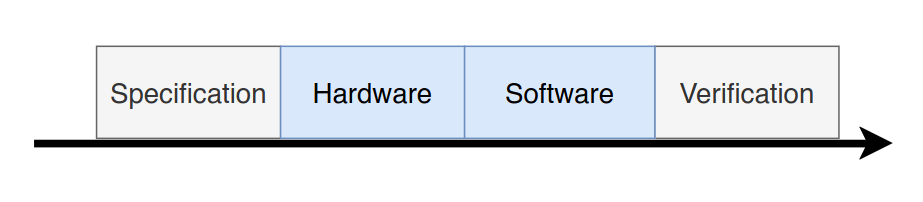
\includegraphics[width=\linewidth]{figures/Virtual_platform_without.png}
        \caption{\ac{SoC} development without virtual platform}
        \label{fig:virtual_platform_without}
    \end{subfigure}
    \vspace{1em}
    \begin{subfigure}[t]{0.8\linewidth}
        \centering
        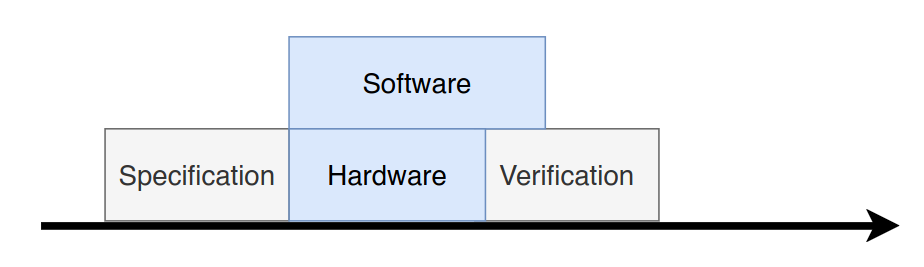
\includegraphics[width=\linewidth]{figures/Virtual_platform.png}
        \caption{SoC development with virtual platform}
        \label{fig:virtual_platform}
    \end{subfigure}
    \caption{Comparison of SoC development with and without virtual platform}
    \label{fig:virtual_platform_comparison}
\end{figure}

\section{Performance Profiling Tools}
Performance profiling plays an important role in software development since it helps developers to identify performance bottlenecks. In reality, there are always trade-offs between the amount of information available and the profiling overheads. Currently, there are three main profiling approaches: sampling, hardware performance counters, and instrumentation.

\begin{itemize}
    \item \textbf{Sampling}: This is a less intrusive approach. Metadata about the target software application is collected periodically. The most representative sampling-based profiler is linux perf, also known as perf\_event\cite{de2010new}. 
    \item \textbf{Hardware performance counters}: Most modern hardware has special-purpose registers available for monitoring hardware events, such as cycle counts, memory access, and many more. Linux perf is also capable of utilizing hardware performance counters to identify performance bottlenecks\cite{weaver2013linux}.
    \item \textbf{Instrumentation}: This is the most intrusive approach since extra code is inserted into the application program for the collection of metadata. On the other hand, it can collect fine-grained information. Common profilers using the instrumentation technique include gprof\cite{graham1982gprof} and valgrind\cite{valgrind}.
\end{itemize}

Regarding the profiling of RISC-V architecture, most of the profiling tools are simulator-dependent. The well-known simulators, including Qemu\cite{banbury2021mlperf}, Spike\cite{spike_simulator}, and gem5\cite{binkert2011gem5}, have their own profiling functionalities.